\addchap{Studienalltag}

Mit dem Studium beginnt ein neuer Lebensabschnitt. Es kommen neue Aufgaben und Herausforderungen auf dich zu, die es zu meistern gilt. Auf den folgenden Seiten möchten
wir dir einen Eindruck darüber verschaffen, wie das Studium aufgebaut ist und wie das Lernen an der Uni funktioniert. Lies dir bitte unbedingt auch mal deine Studienordnung~\link{http://www.verw.tu-dresden.de/AmtBek/PDF-Dateien/2016-06/11soBA24.04.2016.pdf}
und die Prüfungsordnung~\link{http://www.verw.tu-dresden.de/AmtBek/PDF-Dateien/2016-06/11poBA24.04.2016.pdf} durch.

\minisec{Module}
Im Verlauf deines Studiums musst du zahlreiche sogenannte Module erfolgreich absolvieren. Ein Modul kann mehrere Lehrveranstaltungen beinhalten. Das können Vorlesungen,
Übungen, Praktika oder auch Seminare sein. Viele Module bestehen nur aus einer Vorlesung und einer dazugehörigen Übung. Du schließt ein Modul ab, indem du die Modulprüfung
bestehst. Eine Modulprüfung kann sich aus einer oder mehreren Prüfungsleistungen (z.B. Klausur) zusammensetzen. Manchmal muss zunächst eine Prüfungsvorleistung erbracht werden, um
überhaupt an einer Prüfung teilnehmen zu dürfen. Für die einzelnen Module ist in der Anlage 2 zur Studienordnung (Modulbeschreibungen) genau geregelt, welche Prüfungsleistungen zu
erbringen sind.
Jedes Modul hat eine ausgeschriebene Anzahl an Leistungspunkten (LP, oft auch Credits oder ECTS-Punkte genannt). Dabei entspricht ein LP einer Arbeitsbelastung von 30 Stunden. Wenn ein Modul 5 LP bringt, heißt das also,
dass über das Semester verteilt 150 Stunden Arbeit anstehen. Diese Arbeitsbelastung setzt sich zusammen aus Präsenzzeit (Zeit, die du tatsächlich in Vorlesungen/Übungen an der Uni verbringst),
Zeit zur Vor- und Nachbereitung der Lehrveranstaltungen (Selbststudium), Prüfungsvorbereitung und der Prüfung selbst. Die Leistungspunkte für ein Modul werden erst dann anerkannt, wenn
die Modulprüfung bestanden ist.

\minisec{Stundenplan}

An der Uni gibt es ein so genanntes Lehrangebot, das kurz vor Beginn jedes Semesters veröffentlicht wird.
Du findest diese bereits nach Semestern sortierte Liste von Lehrveranstaltungen online auf der Seite der Fakultät~\link{https://www.inf.tu-dresden.de/}.
Ab dem zweiten Semester besteht deine Aufgabe darin, dir aus diesem Angebot deinen Stundenplan zu basteln.
Für den Anfang bekommst du jedoch zum Eingewöhnen fertige Stundenpläne von uns, aus denen du dann einfach einen Stundenplan zur Einschreibung in jExam auswählen kannst. Keine Sorge wir machen das bei der ESE gemeinsam mit dir.

\pagebreak

Während Vorlesungen generell einen festen Termin haben, kannst du dich ab dem zweiten Semester flexibel in die Übungen eintragen.
Schreib dich bei jExam~\link{https://jexam.inf.tu-dresden.de/} einfach für die Übungsstunden deiner Wahl ein.
Stellst du später jedoch fest, dass dein Übungsleiter die Qualitäten einer Schlaftablette aufweist oder dir die Übung zu voll ist, zögere nicht die Übung zu wechseln.

Wenn du dir das Lehrangebot anschaust, wirst du auf die Abkürzung SWS stoßen. SWS steht für Semesterwochenstunden und gibt den Zeitaufwand für eine Lehrveranstaltung an.
SWS treffen dabei lediglich eine Aussage über die Präsenzzeit an der Uni. Die Zeit zur Vor- und Nachbereitung wird dabei nicht berücksichtigt.
Die Angabe 1 SWS bedeutet, dass die Lehrveranstaltung während der Vorlesungszeit wöchentlich durchschnittlich 45 min lang gelehrt wird. Eine Lehrveranstaltung mit 4 SWS wird entsprechend
pro Woche 3 Stunden gelehrt. Eine Lehreinheit an der Uni dauert 90 Minuten und wird Doppelstunde (DS) genannt. Eine Veranstaltung mit 4 SWS findet also 2-mal wöchentlich statt.
Etwas komplizierter ist es, wenn eine Lehrveranstaltung tatsächlich nur 1 SWS umfasst. Dann findet die Veranstaltung nur 14-tägig statt und man muss genau schauen, ob die Veranstaltung jeweils in
geraden oder ungeraden Kalenderwochen stattfindet. Im Stundenplan wirst du dann die Bezeichnungen \enquote{1.\ Woche} oder \enquote{2.\ Woche} finden. Diese haben nichts mit den Wochen seit Semesterbeginn zu tun!
\enquote{1. Woche} bedeutet, dass die Lehrveranstaltung in jeder ungeraden Kalenderwoche stattfindet und \enquote{2.\ Woche} steht analog für gerade Kalenderwochen.

\begin{figure}
	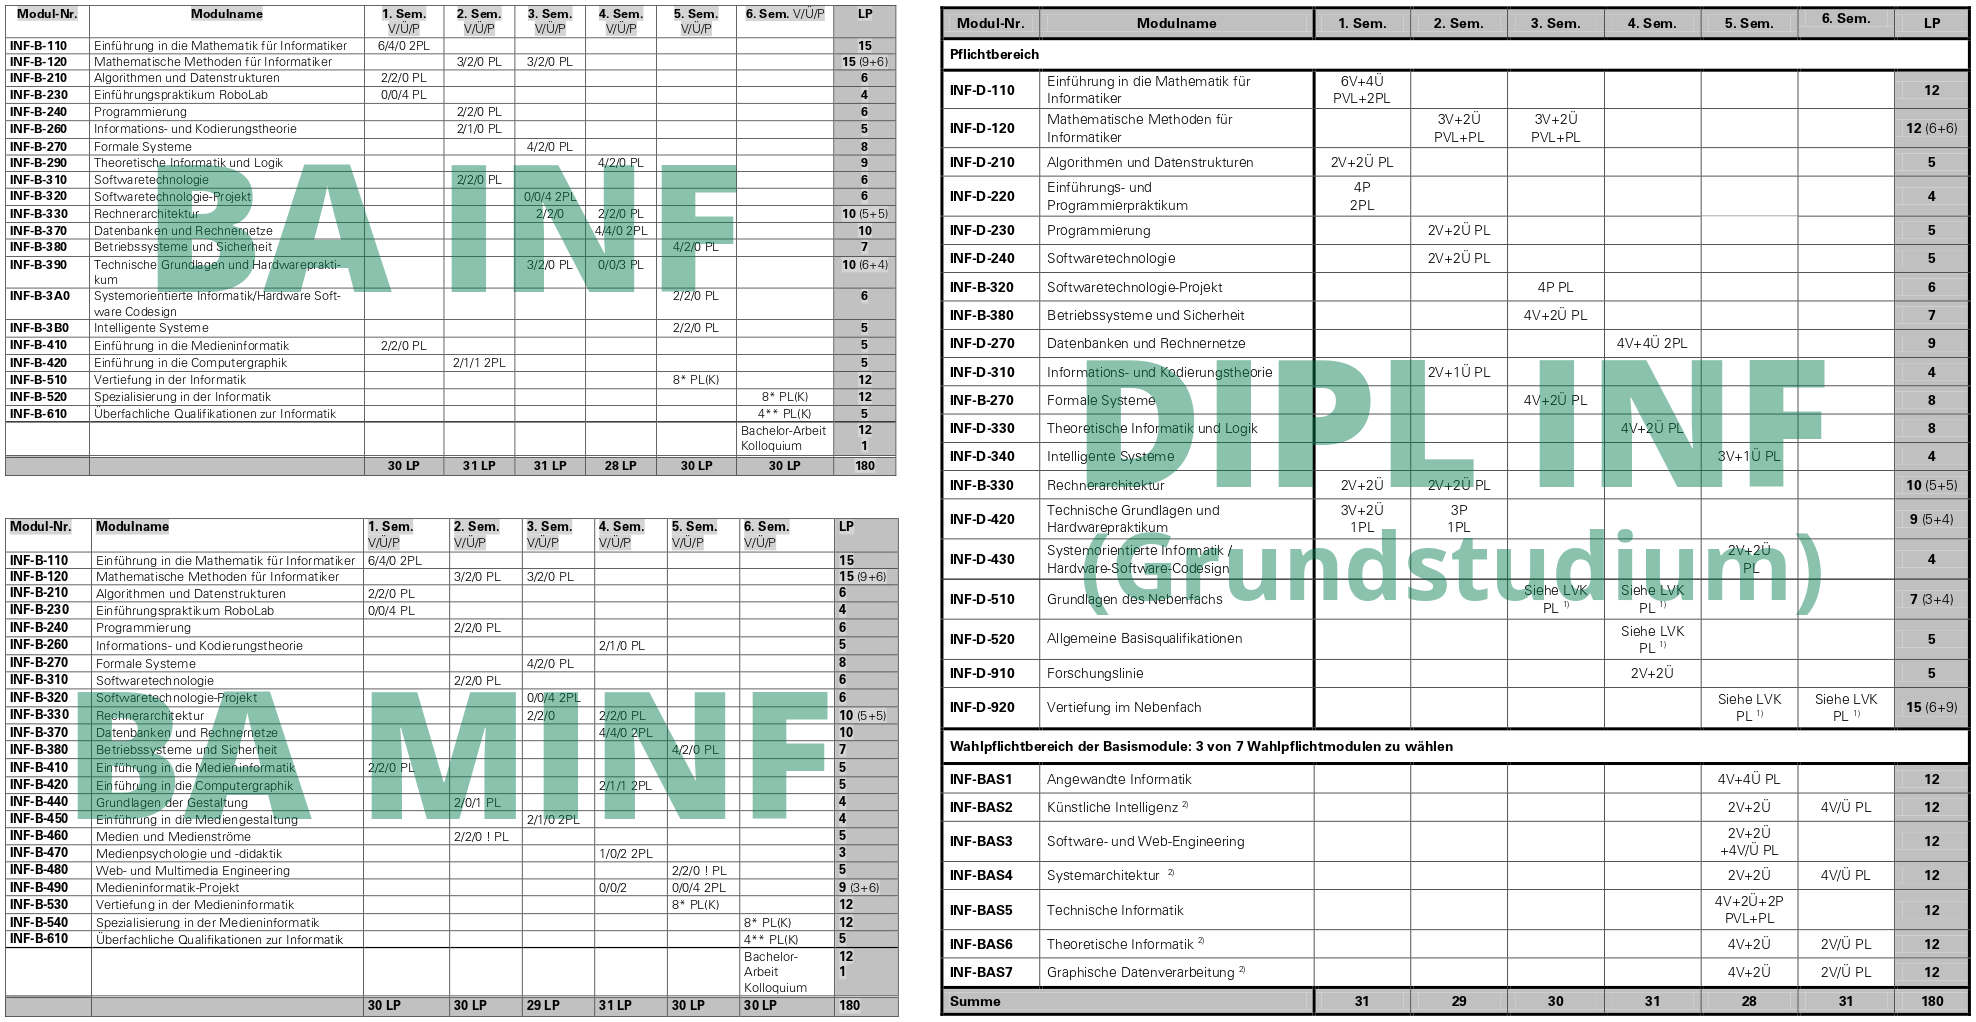
\includegraphics[width=\textwidth]{img/alle_studienablaufplaene.png}
	\caption*{\small \textit{Die Studienablaufpläne aller Studiengänge findest du in groß unter}~\link{https://tu-dresden.de/ing/informatik/studium/studienangebot}.}
\end{figure}

\minisec{Vorlesung}

In den Vorlesungen erlebst du meistens Professoren live.
Die Zahl der Zuhörer ist in der Regel zehn Mal so groß wie die Anzahl der Schüler in einer Unterrichtsstunde. Dadurch kann natürlich nicht auf jeden Studenten eingegangen werden.
Sollte dir jedoch etwas unklar sein, stelle ruhig Fragen. Oft versteht der Großteil der anderen auch nichts.
Außerdem ist es ratsam, dem Stoff stets zu folgen, da die vermittelte Stoffmenge oftmals gewaltig ist. Sich darüber zu beschweren ist sinnlos, da der Lehrplan für die Professoren mehr oder minder vorgeschrieben ist.
Gerade deshalb hat man nur 20 Wochenstunden, da für die Nachbereitung einer Vorlesung mindestens die gleiche Zeit veranschlagt werden sollte.
Über schlechte Tafelbilder, undeutliche und leise Aussprache, sowie mangelnde Vorbereitung der Vorlesung solltest du dich allerdings beschweren.
Professoren sind meist nicht Professoren, weil sie gute Didaktiker sind, sondern weil sie gut forschen können.
Welche Vorlesung du in welchem Semester besuchen solltest, findest du im jeweiligen Studienablaufplan deines Studiengangs
(Bachelor Informatik~\link{https://www.verw.tu-dresden.de/AmtBek/PDF-Dateien/2016-06/11soBA24.04.2016.pdf}, Bachelor Medieninformatik~\link{https://www.verw.tu-dresden.de/AmtBek/PDF-Dateien/2016-06/11soBAMI24.04.2016.pdf}, Diplom Informatik~\link{https://tu-dresden.de/die_tu_dresden/fakultaeten/fakultaet_informatik/studium/dateien/studien_und_pruefungsordnungen/dipl_inf_so_app1_de.pdf}) oder im Vorlesungsverzeichnis auf der Seite der Fakultät~\link{https://tu-dresden.de/ing/informatik/studium/lehre}.


\minisec{Übung}

Übungen werden zu fast allen Vorlesungen angeboten und dienen dazu, Aufgaben zum aktuellen Vorlesungsstoff zu bearbeiten. Klausuren orientieren sich häufig an den Übungsaufgaben, deshalb solltest du die Übungen
regelmäßig besuchen. Die Übungen werden meistens von Studenten aus höheren Semestern oder von Lehrstuhlmitarbeitern gehalten, nicht vom Professor.
Das hat auch den Vorteil, dass man bekanntlich viele Dinge besser versteht, wenn man sie noch einmal aus einem anderen Mund erklärt bekommt.
Die jeweils aktuellen Übungsaufgaben findest du auf der Seite des jeweiligen Dozenten, oft unter den Stichworten Teaching oder Lehre.
Es wird erwartet, dass du dir die Aufgaben bereits vor der Übung anschaust, um dann Lösungen oder Fragen zu diskutieren.


\minisec{Praktikum}

Das erste Praktikum erwartet dich bereits in der vorlesungsfreien Zeit des ersten Semesters -- plane deinen Urlaub also lieber nicht zu schnell!
Dort wirst du im Einführungspraktikum \textit{Robolab} dein Können unter Beweis stellen. Diplomer müssen zusätzlich noch das Strategiespielepraktikum absolvieren.
Ein ganzes Praktikumssemester ist nur für Diplomstudenten im 7. Semester Pflicht.
Natürlich ist es trotzdem empfehlenswert, Praktika bei echten Firmen außerhalb der Fakultät in den Semesterferien zu machen, das steigert nicht nur deine Jobchancen,
sondern zeigt dir auch, ob deine Studienwahl tatsächlich die Richtige war.

\refstepcounter{dummy}\label{sec:pruefungen}
\minisec{Prüfungen}
Direkt an die Vorlesungszeit schließt die Prüfungszeit an – die wohl stressigste Zeit im Leben eines Studenten.
Die genauen Prüfungstermine findest du für das Wintersemester meist etwa Anfang Januar auf der Homepage der Fakultät~\link{https://tu-dresden.de/ing/informatik/studium/news} oder direkt beim Prüfungsamt~\link{https://tu-dresden.de/ing/informatik/studium/pruefungsorganisation}.
Im Laufe des Semesters hast du die Gelegenheit, dich dafür (innerhalb der Einschreibefrist) über jExam einzuschreiben.
Dort hast du auch die Möglichkeit, dich bis zu drei \emph{Werk}tage vor der Prüfung wieder auszutragen. Du kannst die Prüfung auch in einem späteren Semester schreiben.Das sollte aber natürlich nicht zum Regelfall werden. Für mündliche und sonstige Prüfungen gilt eine Abmeldefrist von 14 Tagen.
Solltest du aufgrund eines Rücktritts innerhalb der Frist oder einer plötzlichen Erkrankung von der Prüfung ausscheiden, kannst du dich auf der Seite des Prüfungsamtes informieren,
welche Nachweise (Atteste) du im Prüfungsamt innerhalb welcher Frist einreichen musst~\link{https://tu-dresden.de/ing/informatik/studium/pruefungsorganisation/pruefungen/abmelden-ruecktritt-krankheit}.
Prüfungen werden mit Noten bewertet, wobei alle mit besser als 5.0 bewerteten Prüfungen als bestanden gelten und nicht wiederholt werden können.
Noten Schlechter als 5.0 gibt es nicht.
Die 5.0 ist damit die einzige Chance, eine Prüfung nicht zu bestehen.
Hast du das erst einmal geschafft, gibt es die Möglichkeit, die Prüfung innerhalb von zwei Semestern zu wiederholen.
Nach dem zweiten nicht geglückten Prüfungsversuch hast du nur noch ein Semester Zeit bis der dritte erfolgen muss.
Erst wenn du das dritte Mal die Klausur nicht bestanden hast (also die zweite Wiederholungsklausur), wirst du exmatrikuliert.
Genauere Informationen zu dieser Thematik findest du stets in der Prüfungs- bzw.\ der Studienordnung, die du dir unbedingt mal angeschaut haben solltest.
Deine erste Matheprüfung erwartet dich übrigens bereits im Dezember: die sogenannte Nikolausklausur.

\begin{figure}
	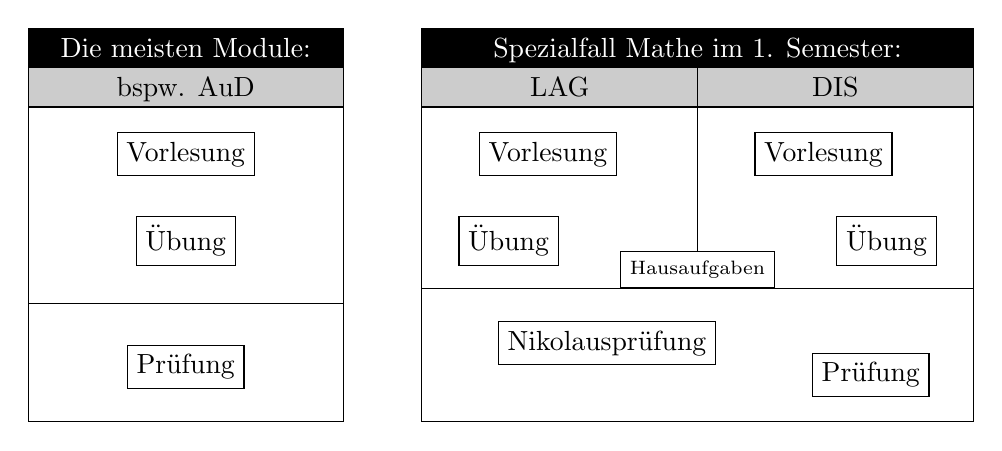
\begin{tikzpicture}
		\draw (0,0) rectangle (4,-5);
		\draw (0,0) [fill=black] rectangle (4, -.5);
		\node at (2,0) [below] {\textcolor{white}{Die meisten Module:}};
		\draw (0,-.5) [fill=gray!40] rectangle (4,-1);
		\node at (2,-.5) [below] {bspw. AuD};
		\draw (0,-.5) -- (4,-.5);
		\node (v1) [draw] at (2,-1.6) {Vorlesung};
		\node (u1) [draw] at (2,-2.7) {Übung};
		\draw (0,-3.5) -- (4,-3.5);
		\node (p1) [draw] at (2,-4.3) {Prüfung};

		\draw (5,0) rectangle (12, -5);
		\draw (5,0) [fill=black] rectangle (12, -.5);
		\node at (8.5,0) [below] {\textcolor{white}{Spezialfall Mathe im 1. Semester:}};
		\draw (5,-.5) -- (12,-.5);
		\node (pvl) [rectangle,draw,font=\scriptsize] at (8.5,-3.3) [above]{Hausaufgaben};
		\draw (8.5,-.5) -- (pvl);
		\draw (5,-.5) [fill=gray!40] rectangle (8.5,-1);
		\node at (6.75,-.5) [below] {LAG};
		\draw (8.5,-.5) [fill=gray!40] rectangle (12,-1);
		\node at (10.25,-.5) [below] {DIS};
		\draw (5,-1) -- (12, -1);
		\node (v2) [draw] at (6.6,-1.6) {Vorlesung};
		\node (u2) [draw] at (6.1,-2.7) {Übung};
		\node (v3) [draw] at (10.1,-1.6) {Vorlesung};
		\node (u3) [draw] at (10.9,-2.7) {Übung};
		\draw (5,-3.3) -- (12,-3.3);
    \node (p2) [draw] at (7.35,-4) {\enquote{Nikolausprüfung}};
		\node (p3) [draw] at (10.7,-4.4) {Prüfung};
		%\draw[->,thick] (pvl) -- (p3);
	\end{tikzpicture}
\end{figure}

\newpage

\minisec{Leistungsnachweis}

Bei manchen Prüfungen erhältst du neben der Note einen Leistungsnachweis (oder kurz: Schein).
Dazu zählen unter anderem die Sprachkurse, die Forschungslinie und z.T. Nebenfachprüfungen. Diese Scheine brauchst du, um dir diese Leistungen im Prüfungsamt anrechnen lassen zu können.

\refstepcounter{dummy}\label{sec:sprachausbildung}
\minisec{Sprachausbildung}

Es werden an der TU Dresden Kurse für fast alle möglichen (und unmöglichen) Sprachen angeboten.
Zu diesem Zweck gibt es zwei Zentren für die Sprachausbildung: Das \enquote{Lehrzentrum Sprachen und Kulturen} (LSK) und \enquote{TUD Institute of Advanced Studies} (TUDIAS).
Das Sprachangebot der beiden Einrichtungen ähnelt sich sehr stark.
Du hast für diverse Sprachkurse ein Budget an Semesterwochenstunden (insgesamt 10 SWS), die du ausgeben kannst, wie du willst.
Für dein Studium zum Bachelor der (Medien-)Informatik sind Sprachkurse generell optional, aber auf jeden Fall empfehlenswert.
Für Diplomstudenten sind 2 Semester Englisch im Laufe des Studiums Pflicht.
Studierst du allerdings Bachelor Informatik und möchtest danach mit dem Master Informatik an der TU Dresden weitermachen, wirst du für den Master das Sprachniveau B2 in Englisch nachweisen müssen,
also kann es sich auch für dich anbieten, die entsprechenden Sprachkurse zu besuchen.
Die Einschreibung für einen Sprachkurs erfolgt online~\link{http://sprachausbildung.tu-dresden.de} mit deinem ZIH-Login.
Sobald die Kurse freigeschaltet sind, solltest du dich jedoch stark beeilen, denn die beliebten Kurse sind meist innerhalb weniger Minuten voll.
Weitere Infos findest du unter~\link{https://tu-dresden.de/lsk/lskonline}~und~\link{http://www.tudias.de/de/Sprachschule.html}.

\vfill
\begin{center}
  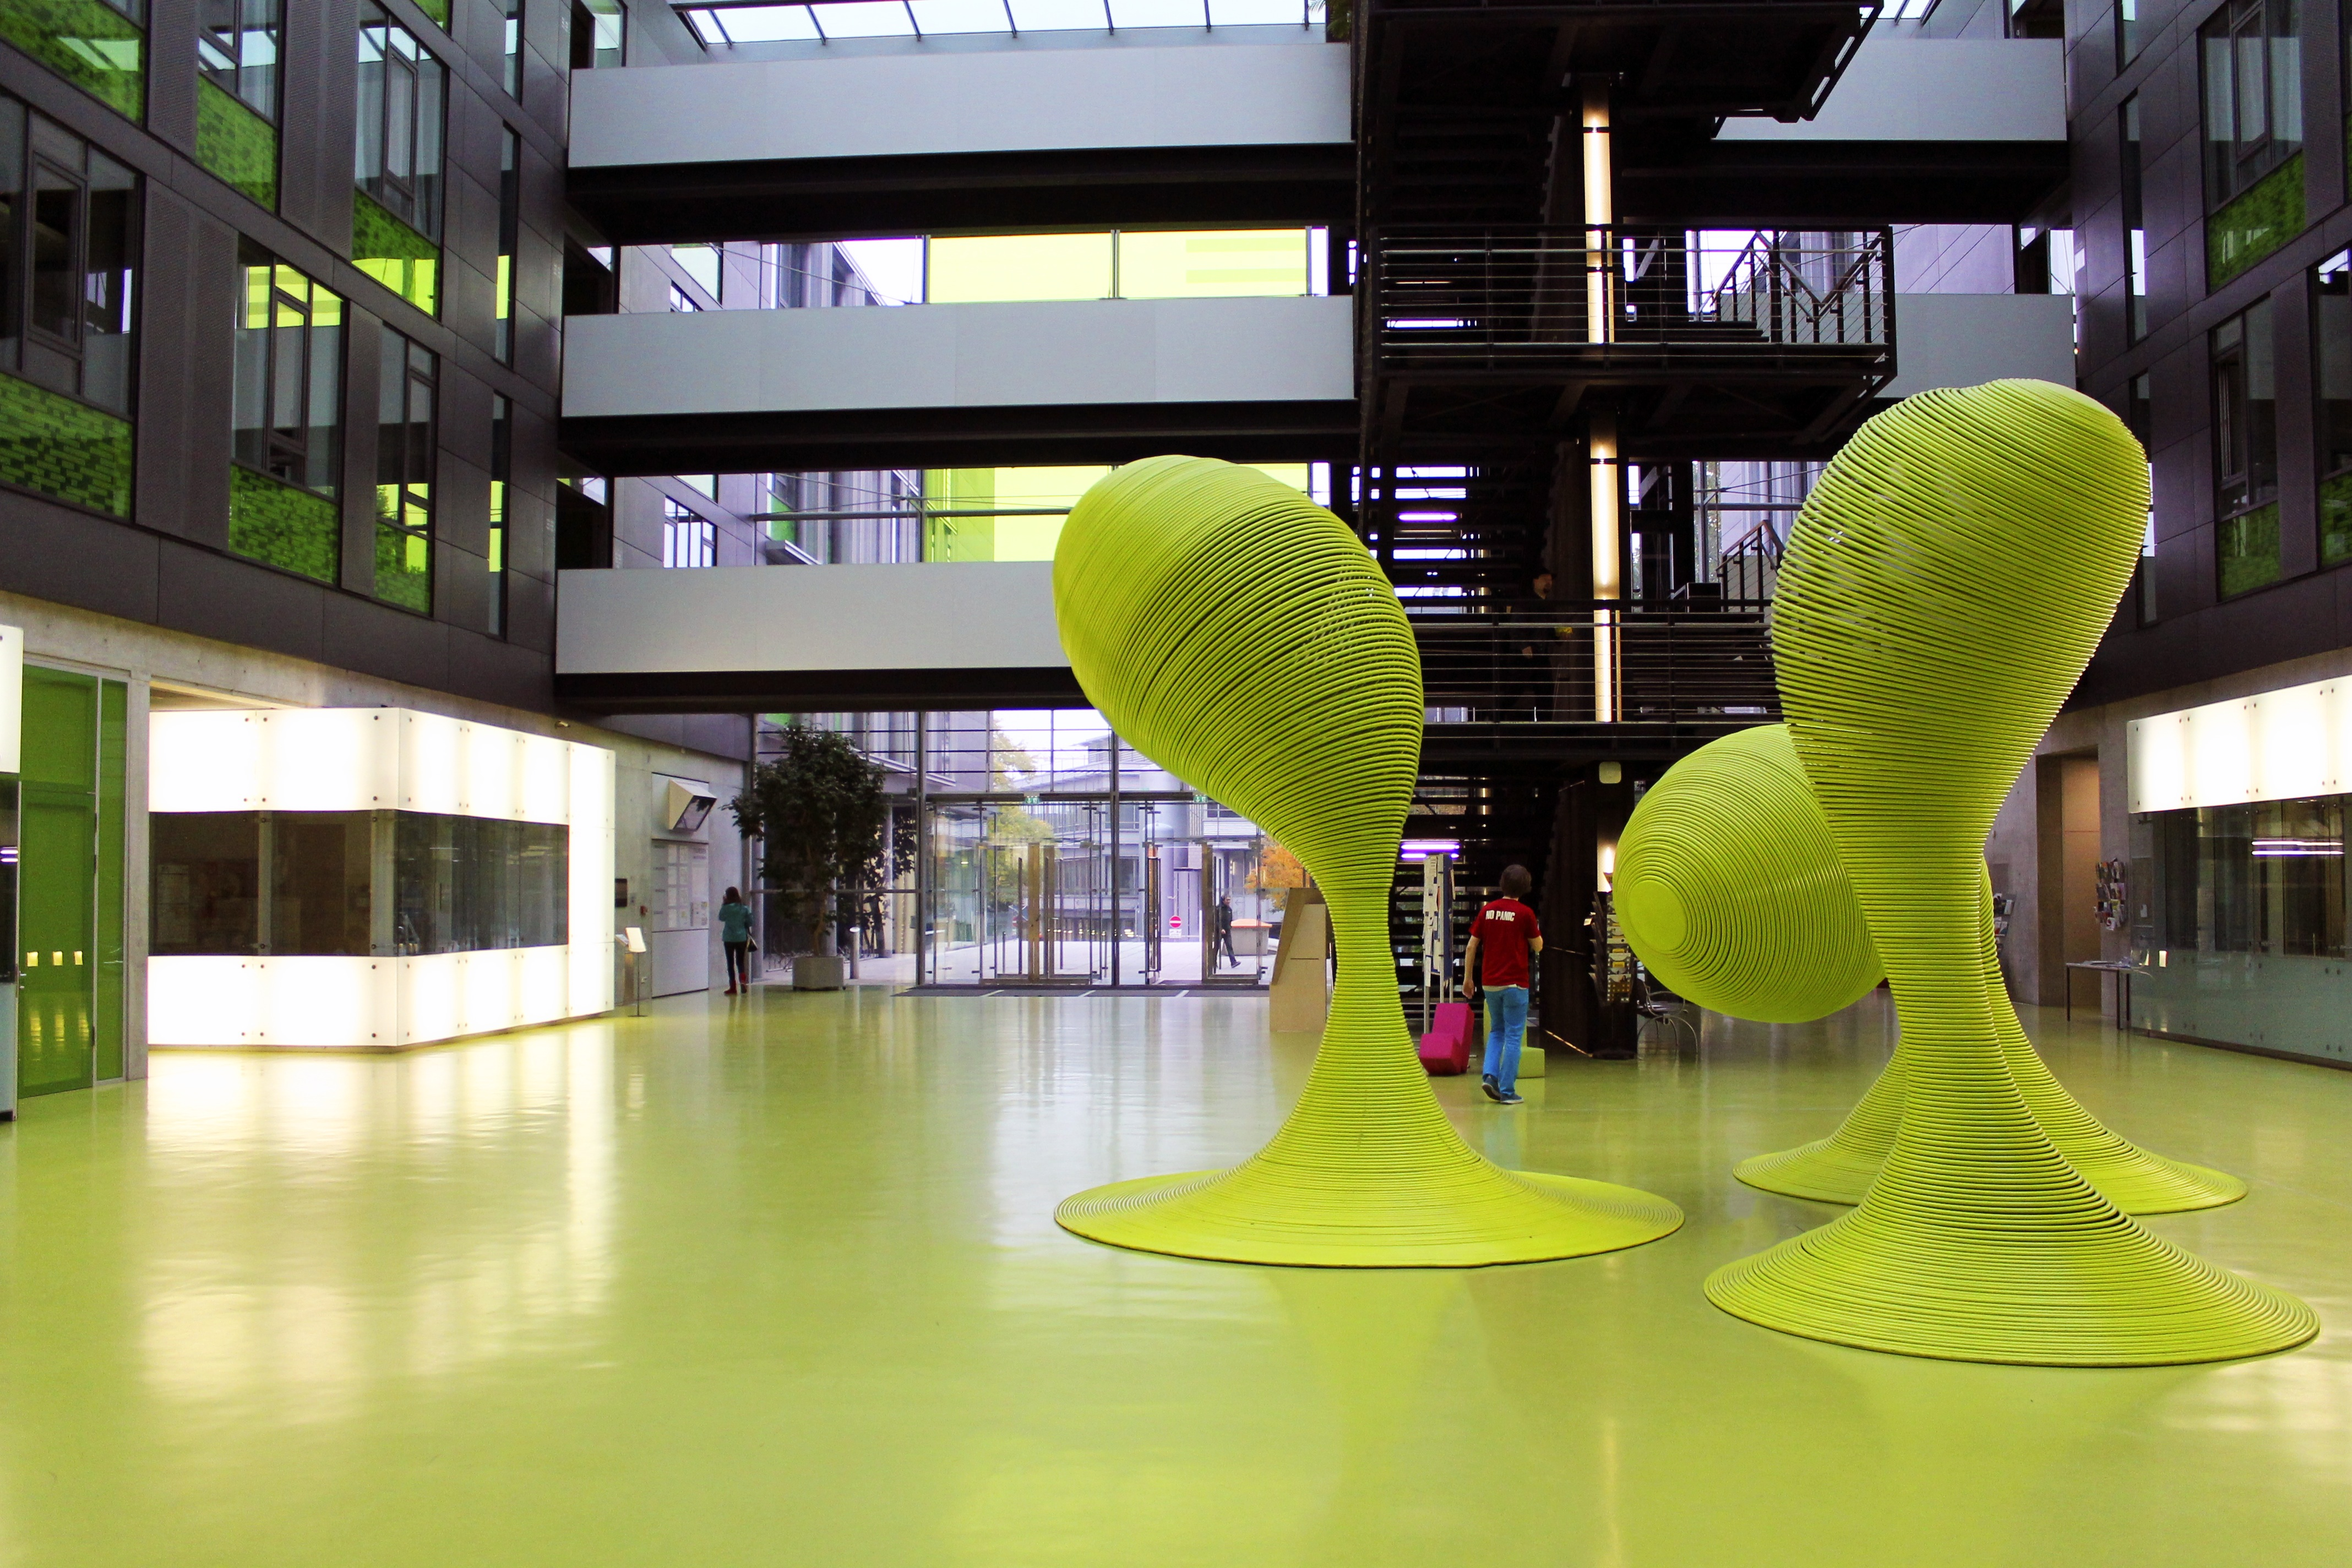
\includegraphics[trim={0 4cm 0 0}, clip, width=\linewidth]{img/ese2013/foyer.jpg}
\end{center}

\minisec{Schreibberatung}
Das Schreibzentrum der TU Dresden~\link{https://www.facebook.com/SchreibzentrumTUD} ist ein Kooperationsprojekt für Studierende und Lehrende vom Zentrum für Weiterbildung und dem Career Service. Es bietet Unterstützung, Methoden und Ideen zum Thema \enquote{wissenschaftliches Schreiben}.
du kannst mit deinen Schreibprojekten aller Art (Beleg, Seminararbeit, Abschlussarbeit, etc.) entweder in die offene Schreibsprechstunde am SCS ServicePoint der SLUB kommen (Dienstags 11:15--12:15 Uhr) oder einen individuellen Termin per E-Mail~\link{mailto:Schreibzentrum@mailbox.tu-dresden.de} vereinbaren.
Dabei spielt es keine Rolle, wie weit die Arbeit bereits ist, ob man also noch ganz am Anfang steht oder kurz vor der Abgabe.
Auch muss kein konkretes Problem vorliegen, sondern intuitive Anliegen zur Arbeit können ebenfalls geschildert werden.

Die Schreibberatung unterstützt bei Fragen zum Schreibprozess -- von der Themenfindung, über die Gliederung bis hin zur Abgabe der fertigen Arbeit.
Ausgebildete studentische Schreibtutorinnen und Schreibtutoren unterstützen dich mit vielfältigen Schreibmethoden und Techniken.
Inhaltliche Tipps oder Hilfestellungen können dir dabei nicht gegeben werden.
Auch liest die Schreibberatung keine Texte Korrektur; allerdings kannst du exemplarisch Textfeedback auf Textauszüge bekommen.
Das Angebot ist selbstverständlich kostenlos.

\minisec{Stipendien}

Neben dem BAföG sind auch Stipendien eine gern genutzte Möglichkeit der Studienfinanzierung.

Viele Stipendien werden von den 13 überwiegend staatlich finanzierten Begabtenförderungswerken vergeben, die sich hinsichtlich ihres weltanschaulichen, religiösen oder politischen Profils unterscheiden.
Oftmals werden Studierende aufgrund guter Leistungen von Schulen, Prüfungsämtern oder Hochschullehrern direkt vorgeschlagen.
Bei vielen Werken sind aber auch Selbstbewerbungen möglich.
Für die Aufnahme muss man keineswegs ein Überflieger sein.

Im Auswahlprozess können gesellschaftliches oder soziales Engagement eine ebenso wichtige Rolle spielen.
Die Stipendien werden in Anlehnung an das BAföG abhängig vom eigenen Einkommen und Vermögen sowie vom Einkommen der Eltern berechnet.
Zusätzlich erhalten die Stipendiaten eine monatliche Studienkostenpauschale in Höhe von 300 Euro.
Im Gegensatz zum BAföG müssen die Stipendien jedoch nicht zurückgezahlt werden.
Neben der finanziellen Förderung bieten alle Werke eine umfangreiche ideelle Förderung in Form von Sprachkursen, Exkursionen und Akademien.

Ebenso bekannt ist das Deutschlandstipendium, welches zur Hälfte von privaten Geldgebern finanziert wird.
Die finanzielle Förderung erfolgt unabhängig vom eigenen Einkommen oder dem der Eltern und beläuft sich auf 300 Euro monatlich.
Das Deutschlandstipendium wird nicht auf das BAföG angerechnet und muss ebenfalls nicht zurückgezahlt werden.
Bewerbungen werden jeweils im Juli direkt vom Zentrum für Weiterbildung der TU Dresden~\link{https://tu-dresden.de/deutschlandstipendium} entgegengenommen.

Es gibt noch viele weitere Organisationen, deren Förderung überwiegend privat finanziert wird. Diese vergeben jedoch oft nur wenige Vollstipendien oder beschränken die Förderung auf geringere Sach- oder Geldleistungen.
Einen Überblick über die Vielzahl an Förderungsmöglichkeiten kann man mithilfe der Stipendiendatenbank des BMBF~\link{https://www.stipendienlotse.de} erhalten.

\begin{figure}[b]
	\centering
	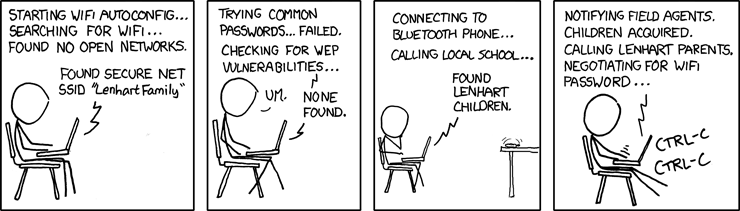
\includegraphics[width=\textwidth, keepaspectratio]{img/xkcd/zealous_autoconfig.png}
	\caption*{{\small \textit{I hear this is an option in the latest Ubuntu release. (https://xkcd.com/416)}}}
\end{figure}

\minisec{Hochschulgruppen}

Lernen und feiern reicht dir nicht?
Such dir eine Hochschulgruppe!
Dort findest du ehrenamtlich engagierte Studierende, die aktiv das Leben auf
dem Campus mitgestalten wollen.
Und je nachdem was du suchst wirst du auch Diskussionen, die Möglichkeit anderen zu helfen, neue Erfahrungen, interessante Leute und vieles mehr finden können.

Thematisch ist für jeden etwas dabei.
So gibt es Hochschulgruppen mit politischem und gesellschaftlichem Engagement.
Andere sind interessiert an der Gestaltung kultureller Vielfalt in Dresden.
Natürlich sind aber auch technisch orientierte Hochschulgruppen vertreten.
Schau dich einfach mal hier~\link{http://www.spirex.de/entfalten/uber-den-tellerrand/hochschulgruppen} um und melde dich direkt bei einer Hochschulgruppe deiner Wahl.
Vielleicht ist ja was für dich dabei.

\minisec{Auslandsaufenthalte}

Bei akutem Auslandswunsch oder studienbegleitendem Internationalisierungsdrang fragen Sie bitte das Auslandsamt der Uni oder Ihren Professor des Vertrauens.
Auslandsaufenthalte können Nebenwirkungen hervorrufen.
Über diese können Sie sich bei Kommilitonen erkundigen.

Im Verlaufe deines Studiums werden dich immer wieder Leute fragen, ob du nicht ein oder zwei Semester im Ausland verbringen möchtest.
Nun magst du dich als unschuldiger Erstsemester fragen, warum denn das und wieso kommt ihr jetzt schon damit an?
Die Antwort ist einfach:
Zum einen kannst du direkt deine Sprachkenntnisse verbessern, Kontakte knüpfen und neue Kulturen erleben -- Eine willkommene Abwechslung, um den Kopf frei zu bekommen nach den anstrengenden Semestern. Es werden neue Perspektiven vermittelt, sowohl akademisch als auch fachlich. Außerdem hilft es dir bei der Entwicklung deiner Softskills wie Selbstständigkeit, Toleranz und Anpassungsfähigkeit (um nur einige zu nennen). Alles Dinge, die dir später weiterhelfen werden und für die du später dankbar sein wirst.
Kurz und knapp gesagt ein Auslandsaufenthalt ist nützlich, erfordert aber etwas Planung.
Deshalb ist es von Vorteil sich möglichst früh zu informieren.
Für Informationen und bei Fragen kannst du dich an das Akademischen Auslandsamts (AAA) der TU~\link{https://tu-dresden.de/studium/im-studium/beratung-und-service/akademisches-auslandsamt} wenden und auf den Seiten der Fakultät~\link{https://tu-dresden.de/ing/informatik/studium/internationales/outgoing} informieren.
Wenn man mutig ist, kann man sogar Professoren direkt fragen, ob sie Kontakte zu anderen Unis oder Unternehmen haben.
Es liegt an dir, wie erfolgreich dein Auslandsaufenthalt wird.
Ob beim Streicheln von Robben vor Neufundland oder beim Scrum-Meeting im Silicon Valley, es gibt so viele Angebote, die man wahrnehmen kann, wenn man sich darum kümmert.

% \begin{figure}[b!]
% 	\centering
% 	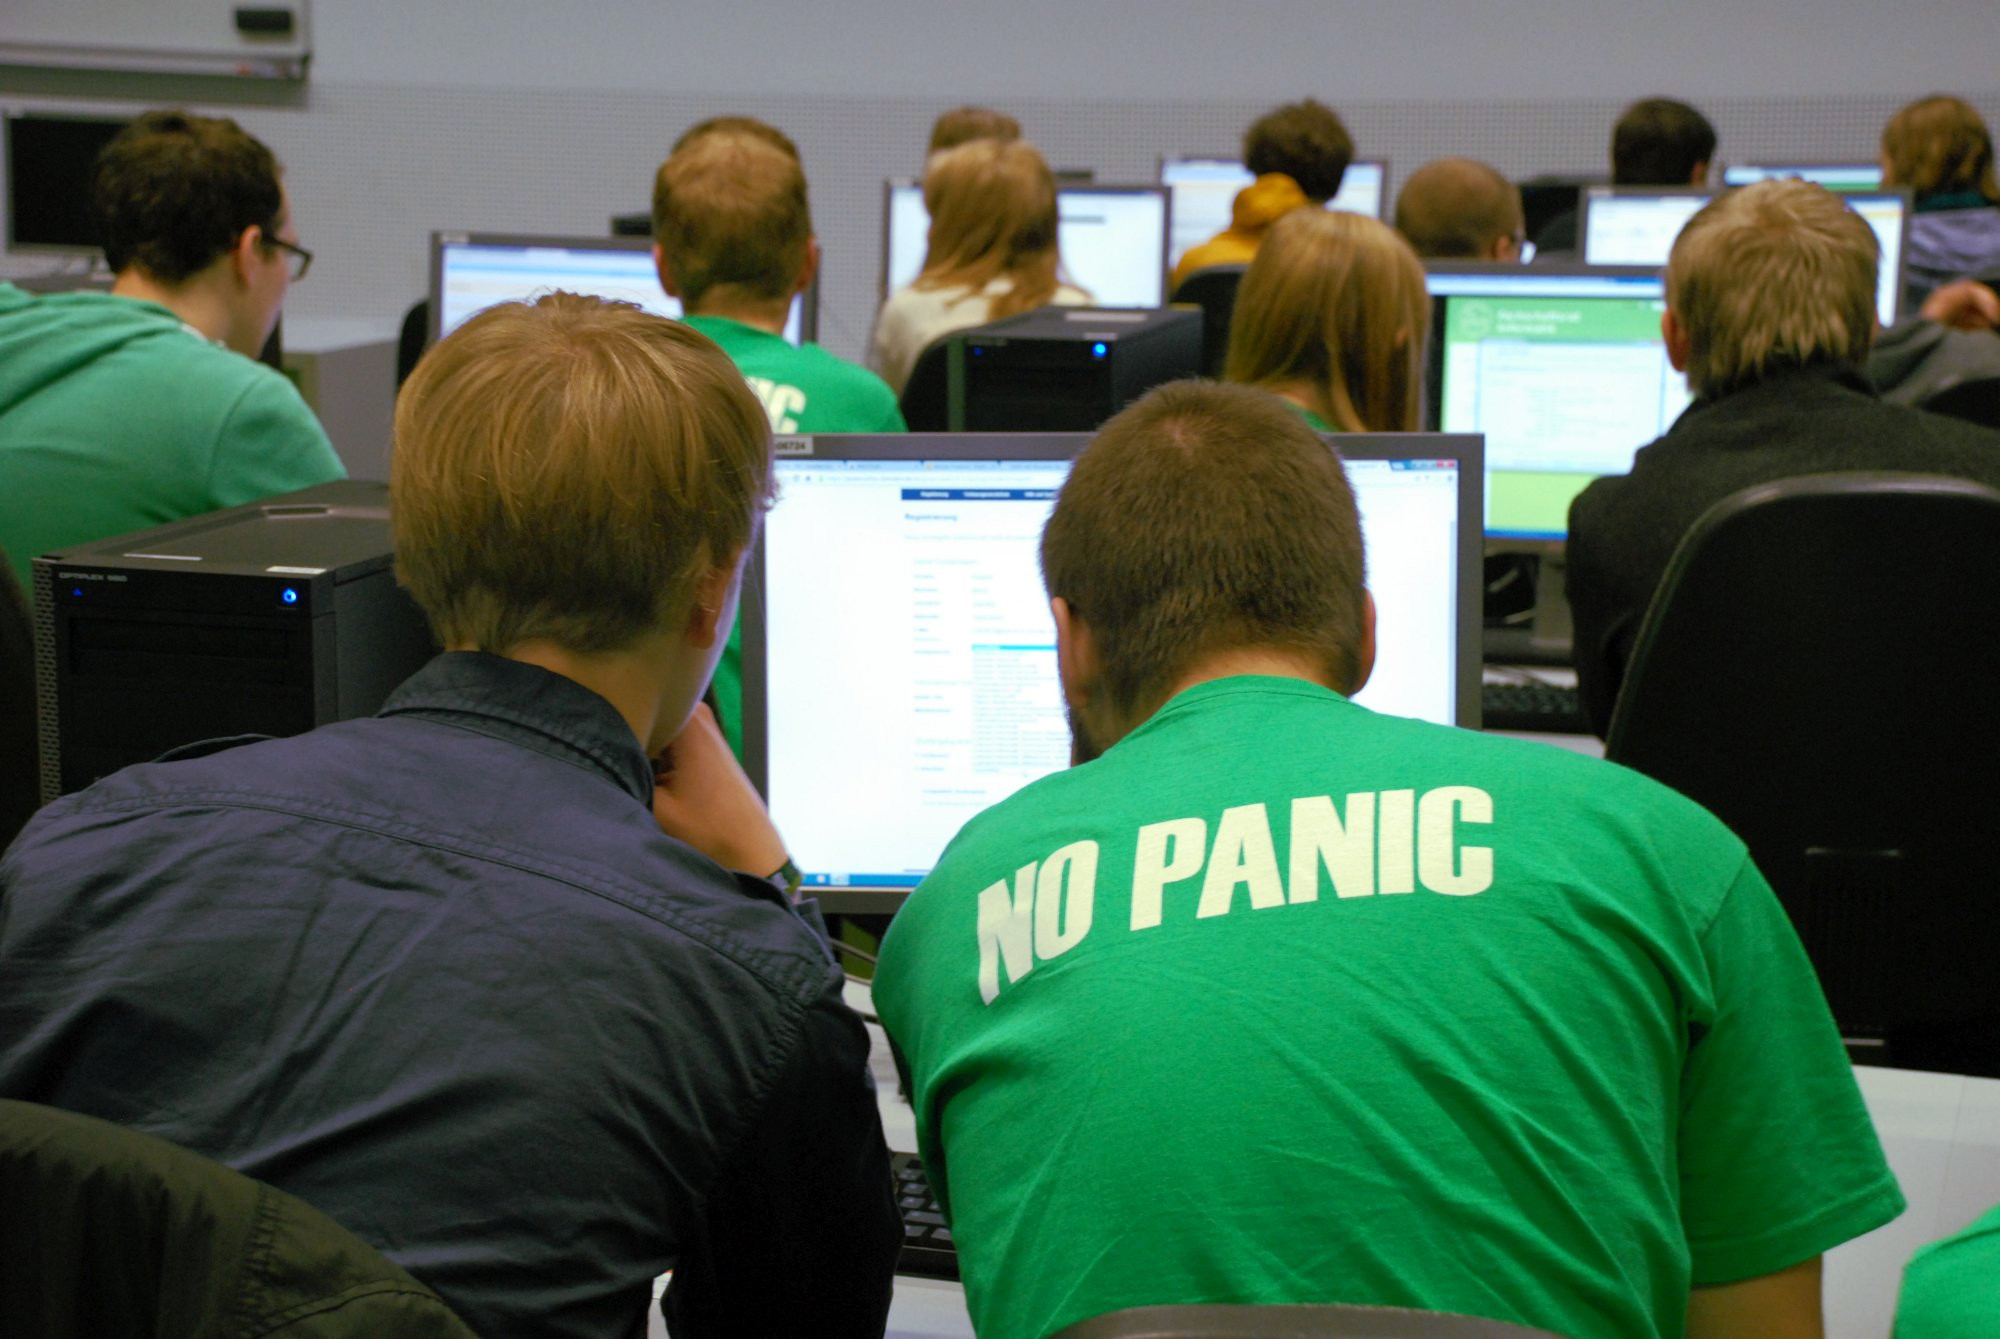
\includegraphics[width=0.9\linewidth]{img/ese2014/einschreibung.jpg}
% \end{figure}%

\minisec{Urlaubssemester}
Es gibt eine ganze Reihe von Gründen, die dich daran hindern können, dein Studium an der TU ordnungsgemäß weiterzuführen.
Klassische Gründe sind schwere Erkrankungen, längere Praktika, Auslandsaufenthalte oder (unverhoffter) Nachwuchs, um den du dich kümmern musst.
In solchen Fällen kannst du dich von deinem Studium beurlauben lassen, um dich voll und ganz auf den Urlaubsgrund zu konzentrieren.
Während eines Urlaubssemesters bist du von der Pflicht befreit, Prüfungen ablegen zu müssen, genießt aber weiterhin alle Vorteile des Studierendendaseins.
Andererseits hast du in dieser Zeit meist auch keinen Anspruch auf BAföG- oder Kindergeld-Zahlungen, also plane das nicht unbedingt bei deinen Einkünften ein.

Solltest du ein Auslandsstudium machen und ein paar Semester in fernen Landen verweilen, kannst du dir danach erbrachte Leistungen und Prüfungen hier anrechnen lassen.
Einziger Fallstrick dabei: Wenn du genügend Leistungspunkte einbringst, wirst du trotzdem ein Fachsemester hochgestuft, aber da kann dir die Studienfachberatung weiterhelfen.

Beantragen kannst du ein Urlaubssemester beim Immatrikulationsamt~\link{https://tu-dresden.de/imma/} während der Rückmeldefrist für das nächste Semester.
Wie genau das geht und weitere Informationen findest du unter~\link{https://tu-dresden.de/studium/im-studium/studienorganisation/beurlaubung}.
